\RequirePackage[final]{graphicx} % to allow for graphics to show in draft mode
\documentclass[oneside, a4paper, final]{memoir} % scrreprt | memoir [twocolumn?]
\usepackage[T1]{fontenc}  % encoding, ligature removal works
\usepackage[utf8]{inputenc}
\usepackage[obeyFinal]{todonotes}
\usepackage{ifdraft}
\usepackage{amsmath}
\usepackage{microtype}
\DisableLigatures{encoding = *, family = *}
\newcommand{\TODO}[1]{\todo[size=\tiny]{#1}}
\newcommand\imglabel[1]{\textbf{\textsf{#1}}}
\renewcommand{\rmdefault}{ptm}

\title{
	Assessing the problem of doing proteomics with \mbox{unsequenced organisms\ifdraft{(DRAFT)}{\thanks{This project was held as a Lab Rotation in Bioinformatics,
			as required by the Master program in Computational Biology and Bioinformatics - ETH Z\"urich}}}}
\author{
	\ifdraft{Roger Bermudez-Chacon\\Supervisor: Katja Baerenfaller}
	        {Róger Bermúdez-Chacón\thanks{D-INFK - Computational Biology and Bioinformatics Master program}\\
			 Supervisor: Katja B\"arenfaller\thanks{D-BIOL - Plant Biotechnology Group}}
}
\date{June 10, 2013}

\setlrmarginsandblock{3cm}{2.5cm}{*}
\setulmarginsandblock{2.5cm}{2.5cm}{*}
\checkandfixthelayout

\begin{document}
\maketitle
\setcounter{secnumdepth}{0}
%c \part{p1}, \chapter{c1}, \section{s2}, \subsection{ss1}, \subsubsection{sss1}, \paragraph{p1}, \subparagraph{sp1}

\section{Introduction}
When dealing with unannotated or partially annotated proteomes, protein identif{}ication is often carried out by
%homology comparison against a reference species (or a set thereof).
searching a database containing protein sequences from other species.
%Homology inference by correspondence or similarity between ion spectra is thus
Identif{}ication of a protein from a different species is
often assumed as enough evidence to 
%label 
claim that this particular protein was identif{}ied in
a protein sample.
This work attempts to systematically evaluate at what extent this holds true, by comparing search results of unannotated
proteins extracted from the \mbox{cassava~(\emph{Manihot~esculenta})} root against dif{}ferent annotated databases, including
the reference species \mbox{\emph{Arabidopsis~thaliana}}, the Viridiplantae~database (containing proteins from a large number
of green plants), and the~annotated~proteome of cassava itself.

\section{Materials, Tools and Methods}
\begin{description}
	\item[Data sources]\hfill
		\begin{description}
			\item[Cassava root sample]\hfill\\
				A sample from the cassava root was analyzed with an LTQ-Orbitrap mass spectrometer. The resulting ion spectra were used in the queries.
			\item[Proteome databases]\hfill\\
				For queries against \emph{Arabidopsis~thaliana}, the database \texttt{fgcz\_3702d\_TAIR10}\cite{arabidopsisdb} 
				(from the Functional~Genomics~Center~Zurich (FGCZ), 29.042.854 residues in 71.033 sequences from \emph{Arabidopsis~thaliana} only) was used.
				For queries against Viridiplantae, the database \texttt{fgcz\_viridi\_d}
				(from the FGCZ, containing 2.062.037 sequences, 693.434.028 residues from annotated proteomes
				of many species of ``green plants'' \textendash including \emph{Manihot~esculenta}\textendash) was used.
				For queries against cassava itself, the database	\texttt{P764\_db2\_d} \cite{cassavadb} (entire
				annotated proteome of \emph{Manihot~esculenta} (cassava), 68.888 sequences from 26.812.366 residues) was used.
				A copy of the cassava database, in \texttt{Fasta} format, was also used during the data processing.
		\end{description}
	\item[Tools]\hfill\\
		The queries against all proteome databases were performed using \texttt{Mascot v2.4.1}~\cite{mascot}.
		Additionally, \texttt{BlastP}~\cite{gappedblast, blastp} queries were performed to search for additional homologs when required.

		The results were processed and the data were analyzed with \texttt{R}~\cite{R}. The auxiliar package \texttt{seqinr}~\cite{seqinr} was used to read \texttt{fasta} f{}iles.
	\item[Methods]\hfill\\
		The ion spectra read from the cassava root protein sample was compared in \texttt{Mascot}, by performing MS/MS ions search queries against each of the three databases listed above.

		The occurrence of carbamidomethyl groups and oxidation were used in all queries as f{}ixed and variable modif{}ications, respectively.

		The queries were performed over all entries in each database. \emph{Trypsin} was used as the cleaving enzyme (up to $1$ missed cleavages allowed).
		The peptide and fragment mass tolerances used were $10\ ppm$ and $0.8\ Da$, respectively.

		The score reported for ranking the matches found was $-10\log{P_m}$, being $P_m$ the probability that a match~$m$ happened as a random event.

		\begin{description}
			\item[Search against the \emph{Arabidopsis~thaliana} database]\hfill\\
				The query was restricted to results with a false-positive tolerance (signif{}icance threshold) of at most 0.05, and ion scores of at least 24.

			\item[Search against the Viridiplantae database]\hfill\\
				The query was restricted to results with a signif{}icance threshold of at most 0.05, and ion scores of at least 38.
			\item[Search against the \emph{Manihot~esculenta} database]\hfill\\
				The query was restricted to results with a signif{}icance threshold of at most 0.05, and ion scores of at least 25.
		\end{description}

		The query results were exported from \texttt{Mascot} for further processing as comma-separated text f{}iles with a formatted header including the search parameters and metadata.

		The data processing was coded as an \texttt{R} script. The implementation relies heavily upon regular expression transformations and set operations.
		The data sets were processed as follows:

		\begin{itemize}
			\item Each of the query result f{}iles was parsed into a data structure of the form $[header, data]$, with $header$ being a set of $name, value$ pairs (\emph{dictionary})
			of variables read from the f{}ile header, and $data$ the actual values read from the comma-separated f{}ile section.

			\item The cassava database, provided as a \texttt{Fasta} f{}ile, was read into an \texttt{R} object with sequence information by using the \texttt{R} package \texttt{seqinr}.

			\item Removal of contaminant references and alternative splice specif{}ications was done by regular expression matching against the protein identif{}iers.
			Here, proteins with identif{}iers pref{}ixed with contaminant markers (\texttt{REV\_, ZZ\_, zz|ZZ\_, rr|REV\_}) were f{}iltered out of the results.
			Alternative splice specif{}ications (suf{}f{}ixes matching `\texttt{.[0-9]+}' in the protein identif{}ier) were ignored in Arabidopsis protein descriptors
			by using only the suf{}f{}ix-free identif{}ier in protein comparisons.

			\item The mapping between protein identif{}iers of cassava and Arabidopsis, to infer homology, was done by parsing
			the \texttt{Fasta} descriptors over the whole cassava database. Entries for which homology information between cassava and Arabidopsis
			has been validated comply with the format
			\begin{align*}
				\mathtt{>[\mathbf{cassava\_id}] \mid [PACid] \mid [Annot] \mid [...] \mid [\mathbf{arabidopsis\_id}] \mid [...] \mid [protein\_description]}
			\end{align*}
			and as such, count with both species identif{}iers.
		\end{itemize}
		
		In particular, the following data were extracted:
		\begin{description}
			\item[Query results of the protein sample against the \emph{Arabidopsis~thaliana} database]\hfill
				\begin{enumerate}
					\item Dif{}ferent proteins identif{}ied by the query.
					Performed by listing the unique protein identif{}iers after contaminant removal (ignoring alternative splicing specif{}ication suf{}f{}ixes).
					\item Identif{}ied peptides, and proteins from the cassava database that contain them.
					Performed by listing the unique peptides that satisfy the scoring, signif{}icance and rank conditions def{}ined in the search parameters.
					These peptides are compared in an `all-against-all' af{}f{}ix (substring) search between each peptide and all the entries in the cassava database.
					\item Cassava homologs of the Arabidopsis search results. Performed by listing the proteins from the cassava database whose \texttt{Fasta} descriptor
					refers to any cassava protein returned from the results in 1.
					\item Cassava proteins both containing high-scoring peptides from the query against the Arabidopsis database and being 
					labeled as homologs of the high-scoring Arabidopsis proteins. Performed by a set intersection between the results from~2.~and~3.
				\end{enumerate}

			\item[Query results of the protein sample against the Viridiplantae database]\hfill
				\begin{enumerate}
					\setcounter{enumi}{4}
					\item Dif{}ferent proteins and protein groups identif{}ied by the query.
					Performed by listing unique protein identif{}iers after contaminant removal (ignoring alternative splicing specif{}ication).
					\item Identif{}ied cassava proteins.
					Performed by listing the unique returned proteins from the Viridiplantae database whose protein identif{}ier corresponds to a
					cassava~(\emph{Manihot~esculenta}) protein	(i.e. protein identif{}iers with suf{}f{}ix \texttt{\_MANES}). Since the Viridiplantae database does not
					return protein identif{}iers in the format the cassava database uses, the mapping between results from Arabidopsis and cassava databases
					had to be done by sequence and/or protein description comparison; conflicts were resolved manually when ambiguities were found.
					\item High-scoring protein groups with no proteins in the cassava proteome. Performed by identifying the protein groups with cassava proteins, 
					and removing them from the list of returned protein groups.
					\item Cassava homologs of the proteins in the highest-scoring protein group with no cassava proteins. Performed by ranking the proteins returned by 7.
					and searching for homologs of the highest-scoring protein in \texttt{Blastp}. If no cassava homologs are listed, a search by protein description is performed
					on the cassava database.
				\end{enumerate}
			\item[Query results of the protein sample against the cassava proteome]\hfill
				\begin{enumerate}
					\setcounter{enumi}{8}
					\item Dif{}ferent proteins identif{}ied by the query.
						Performed by listing the unique protein identif{}iers after contaminant removal.
					\item Cassava proteins occurring in the cassava database search and in the homologs inferred from Arabidopsis and Viridiplantae database search.
						Performed by a set intersection between the results from 4., 8., and 9.
				\end{enumerate}			
		\end{description}
\end{description}

\section{Results}
	The results, summarized in Figure 1, were as follows:
	\begin{description}
		\item[Query results of the protein sample against the \emph{Arabidopsis~thaliana} proteome]\hfill
			\begin{enumerate}
				\item The query returned entries for \texttt{29253} dif{}ferent protein/peptide combinations. \texttt{1442} dif{}ferent proteins returned signif{}icant matches.
				After contaminant removal, and ignoring alternative splicing, \texttt{840} proteins from Arabidopsis were found in the query results.
				\item As many as \texttt{13735} protein/peptide entries that satisfy the score, signif{}icance and rank conditions given by the search parameters were found.
				These entries correspond to \texttt{1677} dif{}ferent peptides from the Arabidopsis database.
				These peptides were found in \texttt{1087} dif{}ferent proteins in the cassava database.
				\item \texttt{1297} out of the \texttt{1442} Arabidopsis proteins found in 1. have been mapped to cassava proteins,
				and are thus assumed as conf{}irmed homologs.
				\item The cassava proteins found both by high-scoring Arabidopsis peptide search (2.) and annotated homology (3.) were \texttt{523}
			\end{enumerate}
		\item[Query results of the protein sample against the Viridiplantae database]\hfill
			\begin{enumerate}
				\setcounter{enumi}{4}
				\item \texttt{4990} dif{}ferent proteins (excluding contaminants) from \texttt{652} dif{}ferent protein groups were found.
				\item Only \texttt{24} cassava proteins were returned by the query. These cassava protein identifiers from the Viridiplantae database were
				mapped to the actual cassava database by sequence and/or description comparison. Matches with only \texttt{20} proteins from the cassava database were found.
				\item \texttt{632} out of the \texttt{652} protein groups found in 5. do not have any cassava protein.
				\item From these groups without cassava proteins, the highest-scoring proteins found correspond to phosphopyruvate hydratases (\emph{enolases}).
				The protein with the best match (entry name \texttt{E4MVZ0\_THEHA}) is described in the database as \texttt{mRNA, clone: RTFL01-03-H18 OS=Thellungiella halophila}.
				An additional query against the UniProt\cite{uniprot} database revealed that this protein is part of the phosphopyruvate hydratase complex, and is also related to the
				enolases in the corresponding family and domain databases.

				Since no cassava homologs to this top-score protein were identif{}ied by \texttt{BlastP}, a search by description using both \texttt{enolase} and 
				\texttt{phosphopyruvate hydratase} was performed on the cassava database. \texttt{5} proteins from the cassava database were found.
			\end{enumerate}
		\item[Query results of the protein sample against the cassava proteome]\hfill
			\begin{enumerate}
				\setcounter{enumi}{8}
				\item \texttt{1412} dif{}ferent proteins from the cassava database were found in the query.
				\item None of the proteins occurred in all query results.
			\end{enumerate}			
	\end{description}

	\begin{figure}[h]
{	\centering
	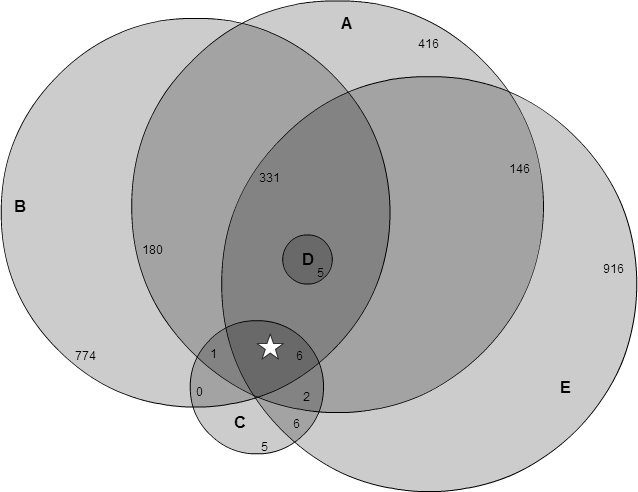
\includegraphics[width=315px]{venn.png}\\}

	\footnotesize Figure 1. Protein distribution for dif{}ferent queries. Each region is labeled with the number of dif{}ferent proteins found on such region exclusively.
	A star denotes the region where the homology assumption is supported by most of the queries.
	%\begin{itemize}
	%\item[A] Cassava proteins containing high-scoring peptides found on the query against the Arabidopsis database.
	%\item[B] Annotated Cassava homologs of the high-scoring Arabidopsis proteins.
	%\item[C] Identif{}ied Cassava proteins found on the query against the Viridiplantae database.
	%\item[D] Cassava homologs of the proteins whose group does not contain Cassava proteins.
	%\item[E] Cassava proteins found on the query against the Cassava database.
	%\end{itemize}

	\imglabel{A} Cassava proteins containing high-scoring peptides found on the query against the Arabidopsis database.\\
	\imglabel{B} Annotated cassava homologs of the high-scoring Arabidopsis proteins.\\
	\imglabel{C} Identif{}ied cassava proteins found on the query against the Viridiplantae database.\\
	\imglabel{D} Cassava homologs of the proteins whose group does not contain cassava proteins.\\
	\imglabel{E} Cassava proteins found on the query against the cassava database.
	\end{figure}
\section{Discussion}
	It is worth noticing from the results above, that no single query returned results supported by all of the others. The region denoted by a star in Figure 1. shows an agreement
	between the possible homologs inferred from the queries against the Arabidopsis database, the cassava proteins found on the Viridiplantae database, and the results
	from the cassava database itself, and is thus the region with the best candidates to annotate the sample.

	The global overlap between results from the Arabidopsis high-scoring peptides (\imglabel{A}), Arabidopsis-cassava annotated homologs (\imglabel{B}), and cassava database results (\imglabel{E}), consists of only up to a third of
	the results returned by each query separately. This number narrows further down when the identified cassava proteins in the Viridiplantae query (\imglabel{C}) are considered. 
	Reliable identification by any of the queries alone is hence not possible.

	In the results from the Viridiplantae database query, protein candidates to label the sample were clustered together in protein groups or families given by protein similarity.
	Some of the high-scoring protein families did not have any cassava protein annotations. Cassava proteins shown as \imglabel{D} in Figure~1. were found
	\textendash via \texttt{BlastP}\textendash\ by similarity search against the highest-scoring protein from those protein groups.
	This best-scoring protein was an \emph{enolase}, and \TODO{surprisingly few cassava proteins were returned. Find out why} none of the 24 cassava
	proteins found against the Arabidopsis database corresponded to neither \emph{enolases} nor \emph{phosphopyruvate hydratases}.

	One obvious next step will be to expand the results from \imglabel{D} to include more results, for example, from cassava proteins similar not to the best-scoring hit only,
	but rather to a large number of high-scoring proteins. The identity and function of cassava protein matches not identified by the query against the Viridiplantae database might
	also be of interest for a future work.

	%Also, since this approach finds protein correspondences 
	%(This reduced group, disjoint to the star, in the future work, include more protein groups.
	%This approach detects correspondences. what about proteins specific to the organism?)
\section{Conclusions}
Since agreement on candidate proteins for sample annotation only occurs on a fraction of the query results, the assumption of correct identification by using a single reference database can definitely 
not be taken for granted. There is overwhelming evidence that protein identification strongly depends on the database chosen for queries. Furthermore, because this approach only tries to find protein
correspondences, the annotation of parts of the protome specific to a given organism still poses a problem.

When possible, it is adviseable to work with fully-annotated proteomes and avoid such assumptions altogether.
However, when this is not an option, one must be very cautious when assuming real interspecies protein correspondences with unannotated proteomes.
\bibliographystyle{ieeetr}  % orders by occurrence in the document
\bibliography{references}
\end{document}
